\documentclass[border=10pt]{standalone}

\usepackage{tikz}
\usepackage{tikzsymbols}
\usetikzlibrary{calc,patterns,shapes.geometric}

\def\centerarc[#1](#2)(#3:#4:#5){\draw[#1] ($(#2)+({#5*cos(#3)},{#5*sin(#3)})$) arc (#3:#4:#5);}

\begin{document}
	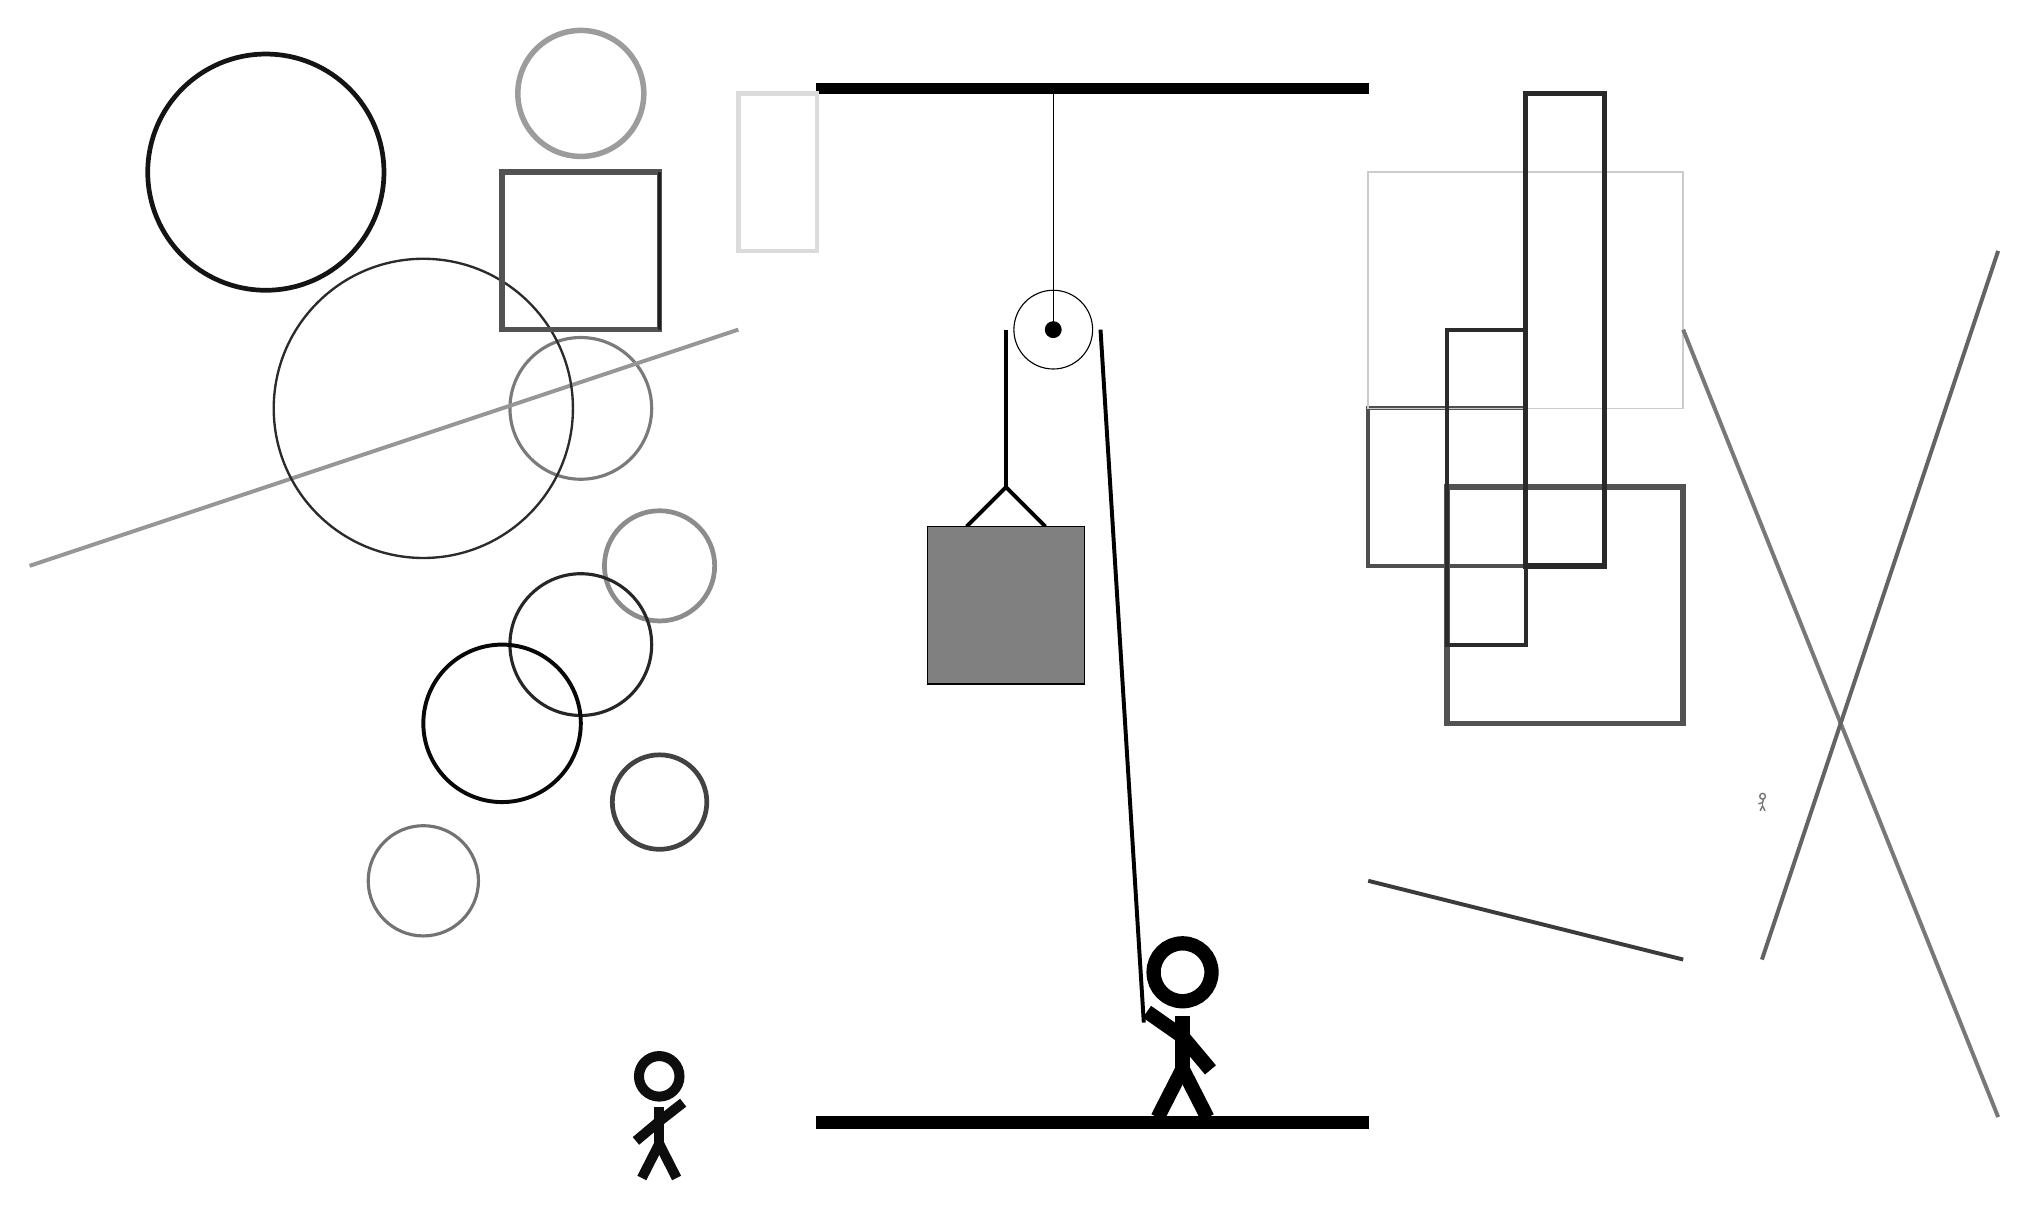
\begin{tikzpicture}
		%%%%% START %%%%%
		
		\draw[fill=black] (-2, 10) rectangle (5, 10.125);
		
		\draw [line width=0.6mm, color=black!92](-9, 9) circle (1.5);
		
		\draw [line width=0.4mm, color=black!55](-7, 0) circle (0.7);
		\draw [line width=0.4mm, color=black!52](-5, 6) circle (0.9);
		\draw [line width=0.6mm, color=black!45](-4, 4) circle (0.7);
		\draw[line width=0.5mm, color=black!69] (5, 6) rectangle (7, 4);
		
		\draw[line width=0.5mm, color=black!21] (-4, 0) rectangle (-4, 0);
		
		\draw [line width=0.6mm, color=black!74](-4, 1) circle (0.6);
		\draw [line width=0.7mm, color=black!87](-6, 2) circle (0.0);
		\draw[line width=0.5mm, color=black!41](-3, 7) -- (-12, 4);
		\draw[line width=0.6mm, color=black!14] (-2, 10) rectangle (-3, 8);
		\draw [line width=0.4mm, color=black!85](-5, 3) circle (0.9);
		\node[line width=0.6mm, color=black!95] at (-4, -3) {\Strichmaxerl[7][40][38]};
		\draw[line width=0.7mm, color=black!68] (6, 5) rectangle (9, 2);
		\draw [line width=0.3mm, color=black!83](-7, 6) circle (1.9);
		\node[line width=0.7mm, color=black!53] at (10, 1) {\Strichmaxerl[1][14][74]};
		\draw[line width=0.2mm, color=black!20] (5, 6) rectangle (9, 9);
		\draw[line width=0.7mm, color=black!68] (-4, 9) rectangle (-6, 7);
		
		\draw[line width=0.5mm, color=black!77](5, 0) -- (9, -1);
		\draw[line width=0.5mm, color=black!83] (6, 3) rectangle (7, 7);
		
		\draw [line width=0.5mm, color=black!97](-6, 2) circle (1.0);
		\draw[line width=0.5mm, color=black!53](9, 7) -- (13, -3);
		
		\draw[line width=0.5mm, color=black!61](10, -1) -- (13, 8);
		\draw[line width=0.7mm, color=black!84] (7, 4) rectangle (8, 10);
		\draw[line width=0.3mm, color=black!88] (-4, 7) rectangle (-4, 9);
		\draw [line width=0.7mm, color=black!39](-5, 10) circle (0.8);
		
		
		\draw (1, 7) circle (0.5);
		\draw[fill=black] (1, 7) circle (0.1);
		\draw (1, 10) -- (1, 7);
		
		\draw[line width=0.5mm] (-0.1, 4.5) -- (0.4, 5.0) -- (0.9, 4.5);
		\draw[fill=black!50] (-0.6, 4.5) rectangle (1.4, 2.5);
		
		\draw[line width=0.5mm] (0.4, 7) -- (0.4, 5.0);
		\centerarc[line width=0.5mm](1, 7)(0:180:0.6);
		\draw[line width=0.5mm](1.6, 7) -- (2.15, -1.8);
		
		\node at (2.6, -1.9) {\Strichmaxerl[10][-35][-50]};
		
		\draw[fill=black] (-2, -3) rectangle (5, -3.15);
		
		%%%%% END %%%%%
	\end{tikzpicture}
\end{document}